\documentclass[UTF8]{ctexart}
\usepackage{graphicx}
\usepackage{lipsum} % 生成示例文本

\begin{document}
\pagestyle{plain}
\lipsum[1] % 示例段落1,\lipsum 是 LaTeX 宏包 lipsum 提供的命令,用于自动生成拉丁文虚拟段落

% 段落间插入浮动图形
\begin{figure}[htbp]%相比center环境的插入方式,figure环境可以让图形浮动,功能也更好,效果更好
    \centering
    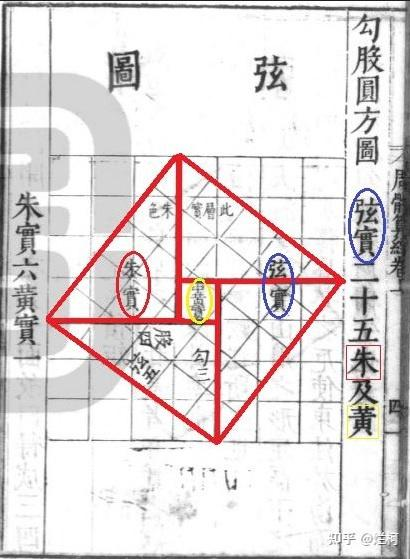
\includegraphics[width=0.5\textwidth]{xiantu.png} % 替换为你的图片路径
    \caption{这是一个浮动图形示例}
    \label{fig:example}
\end{figure}
%center 环境是一个显式的环境,用于将其包裹的内容居中。与 \centering 不同,center 环境会:
%添加额外的垂直间距(类似于 \centering + 上下空白)。
\vspace{2\baselineskip}%两倍当前行高的空白(推荐)

\begin{center}
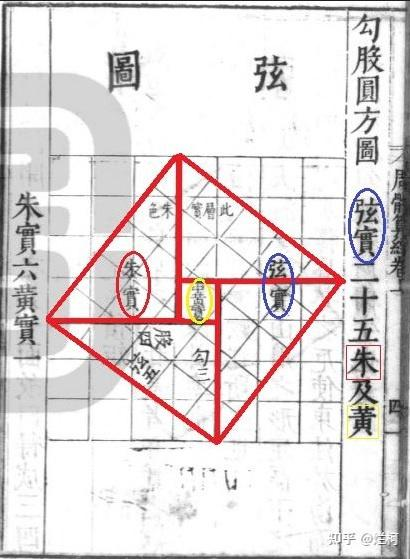
\includegraphics[width=0.5\textwidth]{xiantu.png} % 替换为你的图片路径
\end{center}

\lipsum[2] % 示例段落2

\end{document}